\section{Designing the LUC-OS}
\label{sec:lucos}


% - Section 2: presentation of a reference architecture with challenges 
%   overview.
% - generic architecture -> can be applied to centralized, partially
%   distributed (federation of clouds) and fully distributed (LUC-OS) Cloud OS.
% - LUC-OS design is different of a classical IaaS manager (Controller ->
%   distributed share no state algorithm, DataBase -> DHT, Distributed FS -> p2p
%   FS), this section will expose the development methodology.
Section \ref{sec:moreno} exposed a reference architecture for building a Cloud 
OS, which have been proposed by \cite{moreno2012iaas}: this architecture is 
generic in the sense that it provides a model where each aspect of the Cloud OS 
is managed by a dedicated service. As a consequence, this model can be used as 
well for centralized clouds, partially distributed clouds (federations of 
clouds) and fully distributed clouds. The LUC-OS targets a fully distributed 
functioning, which is not the principal aim of current open-source Cloud 
managers, and thus requires a significantly different architecture oriented 
towards the management of massively distributed clouds.

% - Distributed clouds : hundreds micro DCs, which are themselves composed of up
%   to tens of servers 
% - Managing a distributed cloud -> managing thousands of geographically spread 
%   hosts.
% - P2P file sharing systems: example of software that works well in similar
%   conditions.
% - We think the file sharing systems should be an inspiration for the LUC-OS
%   design.
A massively distributed cloud is an infrastructure that is composed of up to 
hundreds of micro DCs, which are themselves composed of up to tens of servers, 
thus operating such infrastructure means managing up to thousands of
geographically spread servers. Designing software that works at this scale is a
tedious task, as it comes with challenges such as preserving a good reactivity 
and implementing working fault tolerance mechanisms. Peer to peer file sharing 
systems (popular over the last decade) are a good example of software that works
well at large scale in a context where computing resources are geographically 
spread. That is why we propose to learn from the experience of large scale peer 
to peer systems : design rules of the LUC-OS architecture will be directly 
inspired by them. 

\subsection{Design rules}

% - LUC-OS: distributed system: workload divided among every peers.
% - LUC-OS is a multi-agent system: each server (node) of the infrastructure 
%   host one LUC-OS agent.
% - A LUC-OS agent is composed of several services, each service is specialized
%   in a particular task.
% - To prevent bottlenecks and single point of failure, each service is 
%   distributed in a fully distributed manner: 
%    * bottleneck: in case a service is overloaded, it must be able to balance
%      workload on remote service instance.
%    * single point of failure: at large scale, failure becomes the norm rather
%      than the exception, services must implement self healing mechanisms and
%      each persistent state is stored in fault tolerant data structure (DHT).
% - To maximize the reactivity of the LUC-OS, a service should prioritize 
%   collaboration with corresponding services hosted on servers accessible with
%   low latency.
% - To enable low-latency collaborations, each service will leverage a locality
%   based overlay that will dynamically maintain for each server a list of 
%   neighbors.
The LUC-OS targets a fully distributed functioning inspired by the peer to peer
paradigm : its workload will be allocated over among every element constituting
the infrastructure. As we are interested by adding advanced properties 
(self-organization and self-healing) to the LUC-OS, we propose to leverage a 
multi-agent architecture: each node (server) constituting the infrastructure 
will host one of the LUC-OS agent. To prevent negative phenomenons such as
bottlenecks and single points of failure (SPOF), we have decided to anticipate
them during the design stage:

\begin{description}

  \item [Bottlenecks] : are caused by an excessive workload allocated to one 
  service, which slows its interactions with collaborators, thus impacting
  negatively the performance of the infrastructure by reducing both reactivity 
  and quality of service. Indeed, when a service is overloaded, it is better to 
  enable him to distribute the workload on several remote instances that are
  underloaded.

  \item [Single points of failure] (SPOF) represents an element of a system, 
  that in case of failure, stops the entire system. As at large scale, failure 
  becomes the norm rather than the exception, SPOFs are a major concern in
  distributed software: that is why services must implement self healing 
  mechanisms such as redundancy. In addition each persistent state have to be 
  stored in fault tolerant data structure like a distributed hash-table (DHT).

\end{description}

\subsection{Anatomy of a LUC-OS agent}


\begin{figure*}
	\centerline{
	 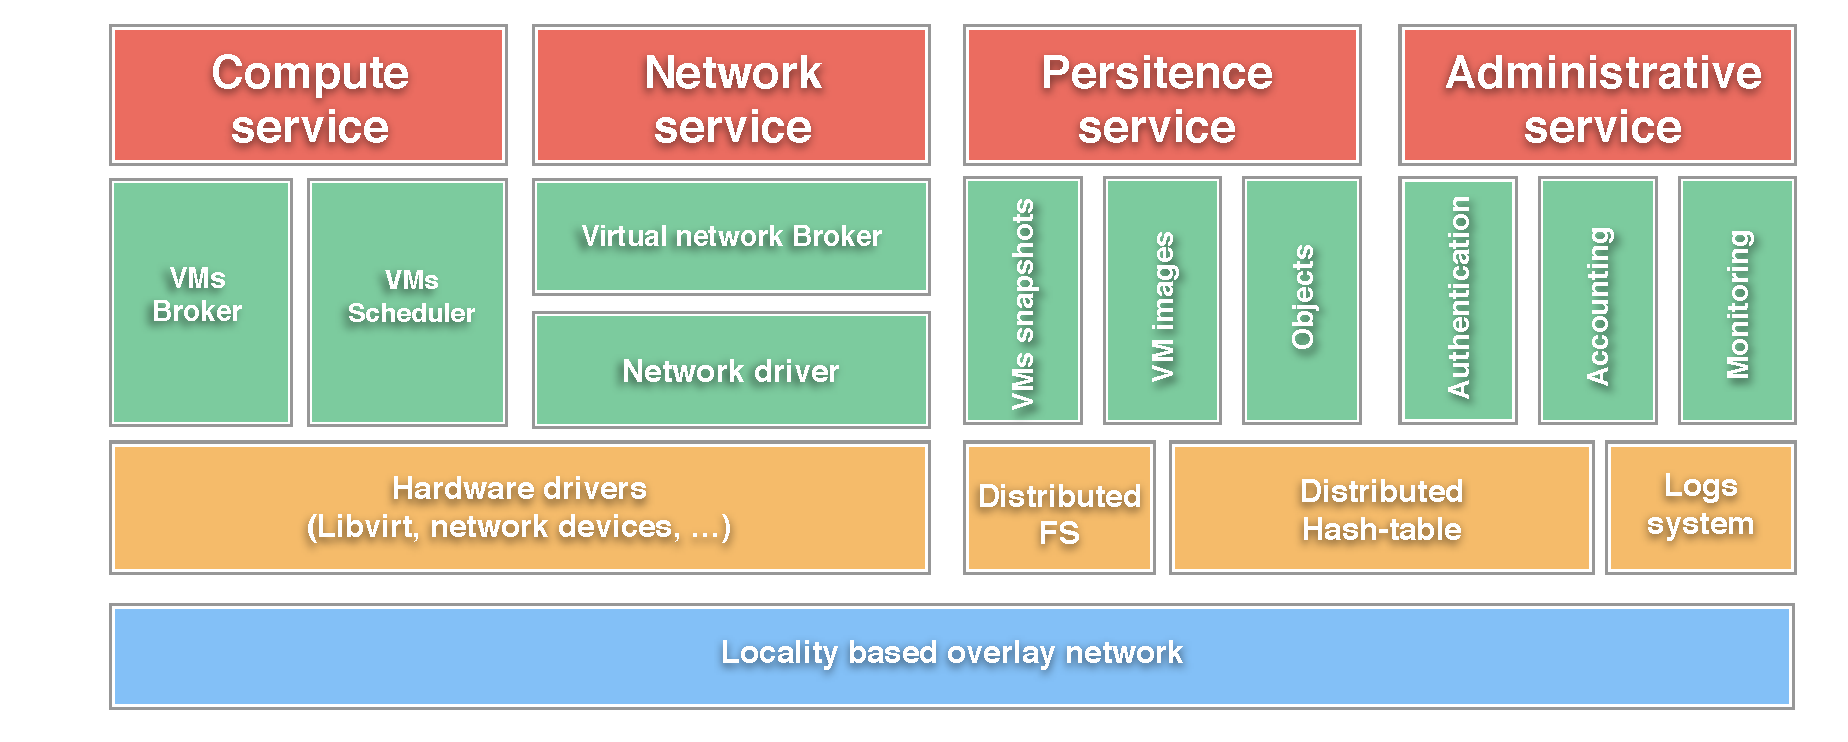
\includegraphics[width=1.25\linewidth]{Figures/luc_os_anatomy.pdf}
  }
	\caption{Anatomy of services composing the LUC-OS.}%
	\label{fig:anatomy}%
	%\vspace*{-.8cm}
\end{figure*}

% - Figure \ref{fig:anatomy} -> our choices
% - 4 services: one service per aspect (compute, network, persistance, admin). 
% - Compute service: delivery of computing resources: built on top of:
%    * VMs broker: receives VM creation request, elect a server: it instantiate 
%      the VM; ensures VM creation.
%    * VMs scheduler: ensures good QoS for VMs: compute node overloaded ->
%      sched balances workload on underloaded ones (dynamic scheduling).
% - Network service: create virtual that interconnect VMs (broker). Network 
%   creation abstracted by the use network drivers (OpenFlow, Mininet, ...).
% - As some services manipulate hardware -> direct access via Hardware Drivers.
% - Persistence service: store states manipulated by the services of the LUC-OS:
%    * Objects (serializable entities); VMs images (VMs template) belonging to a 
%      specific user (+ metadata); VMs snapshots: like VM images with versions.
% - These sub-services leverage a DHT, and some of theme leverage a resilient 
%   distributed FS.
% - Administrative: managing the infrastructure and producing statistical and 
%   usage data.
% - To perform those tasks it will leverage a DHT and a service that store 
%   execution logs of the infrastructure.

\label{sec:anatomy_lucos}
Figure \ref{fig:anatomy} depicts our architectural choices: each aspect of the 
LUC-OS is managed by a specific service that will collaborate with close 
instances of the service located on remote nodes through the use of locality
based network overlay. 

\subsubsection{Compute service}
is in charge of the delivery of computing power: it is built on top of two 
sub-services : \emph{VMs broker} which process requests for VMs creation (static
scheduling: it elects a server that will instantiate the VM and ensures that the
VM is successfully created) and \emph{VMs scheduler} that guarantees a good 
quality of service for VMS by balancing workload of overloaded compute node on
underloaded ones (dynamic scheduling). 

\subsubsection{Network service} 
leverages a \emph{virtual network Broker} that create virtual networks 
interconnecting VMs. Creation of these virtual networks is abstracted by the use
of \emph{Networking drivers}: it enables the use of a wide range of network 
technology such as OpenFlow and Mininet. As all services composing Compute 
service and network drivers manipulate hardware, they will have direct access to
hardware via Hardware Drivers. 

\subsubsection{Persistence service}
is dedicated to keeping states of the LUC-OS by leveraging one service for each
kind of state: \emph{Objects} are used to persist serializable entities 
manipulated by the LUC-OS, \emph{VMs images} are used for VMs template files 
(which belong to a specific user), \emph{VMs snapshots} are pretty much the same
as VM images except that they support versionning. All the sub-services that 
compose the Persistence service leverage a distributed hash-table, and those 
which are in charge of persisting images and snapshots will leverage a resilient 
distributed file system. 

\subsubsection{Administrative service} 
will perform tasks such as managing the infrastructure and producing statistical
and usage data. To perform those tasks it will leverage a distributed hash table
and a service that stores execution logs of the infrastructure.



